\ProvidesFile{JacobianReport.tex}

\documentclass[a4paper]{article}

\makeatletter
\def\ps@myPS{%
    \def\@oddfoot{\null\hfill\thepage}
    \def\@evenfoot{\thepage}%
    \def\@evenhead{\null\hfil\slshape\leftmark}%
    \def\@oddhead{{\slshape\rightmark}}}%
\makeatother

\pagestyle{myPS}

\usepackage{tikz}
\usepackage{epsfig}
\usepackage{afterpage}
\usepackage{floatpag}
\usepackage{color}
\DeclareGraphicsRule{.pdftex}{pdf}{.pdftex}{}

\usepackage{caption}
\usepackage{subcaption}

\usepackage{hyperref}

\usepackage{float}

\usepackage{times}
\usepackage[numbers]{natbib}
\usepackage{graphicx}
\usepackage{url}

\usepackage{amsmath,amssymb}
\usepackage{cases}
\usepackage{a4wide}
\usepackage{tikz}

\begin{document}

\setcounter{page}{1}
\pagenumbering{arabic}

\begin{titlepage}
\begin{center}

{\huge \bfseries Contact Jacobian Computation}

\vspace{2cm} 

\textsc{Jan Michalczyk} \\

\texttt{jan.michalczyk@inria.fr} \\[2cm] 

{March 31, 2014}

\vspace{2cm} 


\includegraphics[width=0.29\textwidth]{INRIA}

\end{center}
\end{titlepage}


\section{Introduction}

This short document explains the computation of the contact jacobian for the exomars rover model. \\

\noindent There are three sections:

\begin{itemize}
  \item First one explains the general way of deriving a geometric jacobian of the manipulator.
  \item Second one explains the particular case of the exomars rover model.
  \item Third one explains an alternative approach of computing the contact jacobian
\end{itemize}

\subsection{General way of comupting a geometric jacobian}

\noindent We consider the general case of a three degree-of-freedom manipulator (as below):

\begin{figure}[h!]
  \centering
    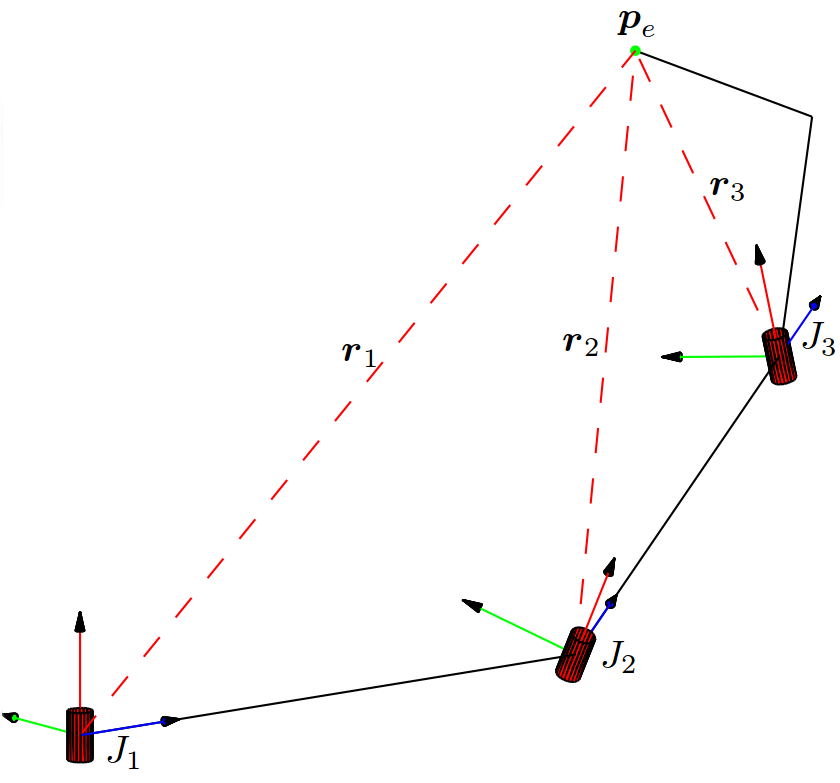
\includegraphics[width=0.8\textwidth]{jacobian}
  \caption{Three DOF manipulator}
\end{figure}

\noindent Where (for \textit{i} = 1,...,3):

\begin{itemize}

\item \textbf{\textit{k}}$_{i}$ - axis of rotation of $J_{i}$
\item \textbf{\textit{r}}$_{i}$ - vector from $J_{i}$ to \textbf{\textit{p}}$_{e}$

\end{itemize}

\noindent \textbf{\textit{k}}$_{i}$ and \textbf{\textit{r}}$_{i}$ are expressed in the global frame. \\

\noindent Then the formula which allows to comupute the velocity of the point \textbf{\textit{p}}$_{e}$ in terms of joint velocities $\dot{\textbf{\textit{q}}}$ is as follows:

\begin{equation}
\begin{bmatrix}
       \boldsymbol{v}_{e} \\
       \boldsymbol{\omega}_{e}             
\end{bmatrix} = \begin{bmatrix}
       \boldsymbol{k}_{1} \times \boldsymbol{r}_{1} & \boldsymbol{k}_{2} \times \boldsymbol{r}_{2} & \boldsymbol{k}_{3} \times \boldsymbol{r}_{3} \\
       \boldsymbol{k}_{1} & \boldsymbol{k}_{2} & \boldsymbol{k}_{3}              
\end{bmatrix} \begin{bmatrix}
       \dot{q}_{1} \\
       \dot{q}_{2} \\
       \dot{q}_{3}             
\end{bmatrix}
\end{equation}

\noindent Where the matrix: \\


\begin{equation}
\underbrace{\begin{bmatrix}
       \boldsymbol{k}_{1} \times \boldsymbol{r}_{1} & \boldsymbol{k}_{2} \times \boldsymbol{r}_{2} & \boldsymbol{k}_{3} \times \boldsymbol{r}_{3} \\
       \boldsymbol{k}_{1} & \boldsymbol{k}_{2} & \boldsymbol{k}_{3}              
       \end{bmatrix}}_{J}
\end{equation}

\noindent is the Jacobian matrix. Entries in the columns depend on the type of the joints. The case above holds when all joints are revolute. In the case the \textit{i}-th joint is prismatic
the respective column should contain the following entry:

\[
\begin{bmatrix}
       \boldsymbol{k}_{i} \\
       \boldsymbol{0}             
\end{bmatrix}      
\]

\subsection{Specific case of the exomars rover model}

\noindent In the figure below we can see the case of the kinematic chain with a wheel at the end of it. We assume that the $J_{1}$ is attached to a base of the rover.  

\begin{figure}[h!]
  \centering
    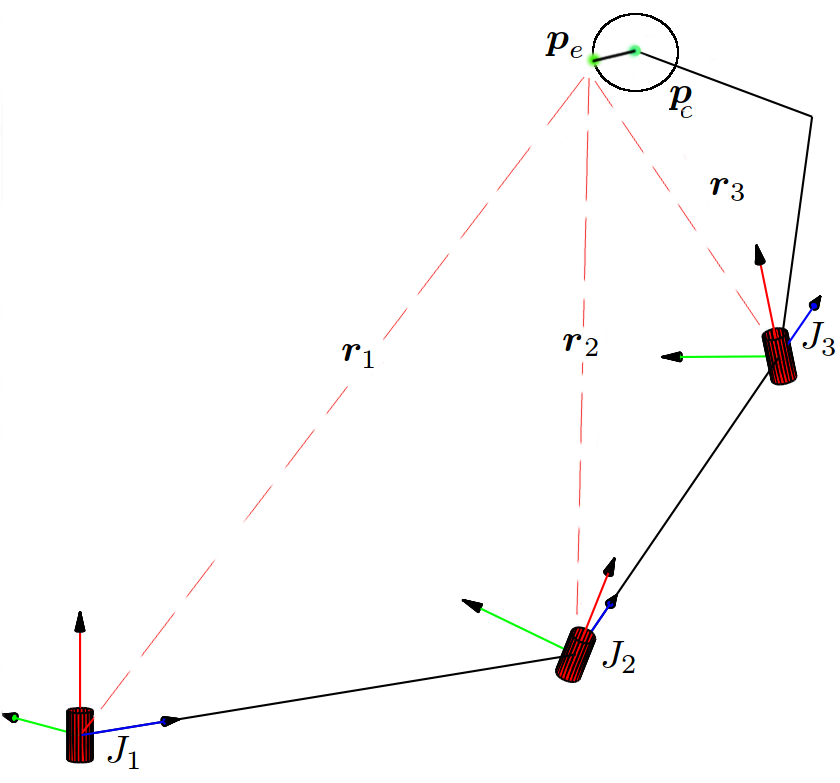
\includegraphics[width=0.8\textwidth]{newjacobian}
  \caption{Three DOF manipulator with a wheel at the end}
\end{figure}

\noindent Kinematic chain as above can represent a simplified version of one of the six chains in the rover model leading from the base down to the respective wheel. To obtain the entries of the jacobian corresponding to the joints of the model ( $q_{6} \ldots q_{20}$ ) coordinates of the joints and joint axes are needed. Those can be obtained from HuMAnS code generator by putting tags in the right places on the model. 
It is also clear from the figure that to obtain the entries of the jacobian the coordinates of the contact point are needed. Those are computed using the normal vector in the contact point given by Trasys API. 
To sum up, last fifteen columns of the jacobian can be computed using the formula (2). As six jacobians need to be computed (one for each wheel), the connectivity of the whole chain needs to be handled. This means that
for every wheel only columns representing joints contributing to the motion are computed, remaining columns are filled with zeroes. Last three rows of the jacobian in the sense of equation (1) can be neglected as we only need 
the part corresponding to the linear velocity. $\boldsymbol{p}_{e}$ is the contact point, whereas $\boldsymbol{p}_{c}$ is the center of the wheel. \\

\noindent From the above considerations we can write down the portions of the jacobian matrices corresponding to the joints $q_{6} \ldots q_{20}$. Base of the rover will be handled separately later on. We remind all joint 
variables of the system's so that subsequent connectivity considerations are clear. 

\begin{itemize}
\item $q_{0}$ - base x coordinate in the global frame
\item $q_{1}$ - base y coordinate in the global frame
\item $q_{2}$ - base z coordinate in the global frame
\item $q_{3}$ - base rotation around x axis
\item $q_{4}$ - base rotation around y axis
\item $q_{5}$ - base rotation around z axis
\item $q_{6}$ - rear bogie joint 
\item $q_{7}$ - rear left steering joint 
\item $q_{8}$ - rear right steering joint
\item $q_{9}$ - rear left wheel joint
\item $q_{10}$ - rear right wheel joint   
\item $q_{11}$ - front left bogie joint 
\item $q_{12}$ - center left steering joint 
\item $q_{13}$ - front left steering joint 
\item $q_{14}$ - center left wheel joint 
\item $q_{15}$ - front left wheel joint 
\item $q_{16}$ - front right bogie joint 
\item $q_{17}$ - center right steering joint 
\item $q_{18}$ - front right steering joint 
\item $q_{19}$ - center right wheel joint
\item $q_{20}$ - front right wheel joint   
\end{itemize} 

\noindent Jacobian for the contact point on the wheel RL (rear left): \\
\noindent (supporting joints: rear bogie joint - $q_{6}$, rear left steering joint - $q_{7}$, rear left wheel joint - $q_{9}$)

\begin{align}
J^{(n)}_{RL} =
\begin{cases}
        \begin{pmatrix} \boldsymbol{k}_{n} \times \boldsymbol{r}_{n, RL} \end{pmatrix} if \ n \in \{6, 7, 9\}\\
        \begin{pmatrix} \boldsymbol{0} \end{pmatrix} \ \ \ \ \ \ \ \ \ \ \ \ \ \ \ \ if \  otherwise
\end{cases}
\end{align}

\noindent Which results in a $3 \times 15$ matrix. \\

\noindent Jacobian for the contact point on the wheel RR (rear right): \\
\noindent (supporting joints: rear bogie joint - $q_{6}$, rear right steering joint - $q_{8}$, rear right wheel joint - $q_{10}$)

\begin{align}
J^{(n)}_{RR} =
\begin{cases}
        \begin{pmatrix} \boldsymbol{k}_{n} \times \boldsymbol{r}_{n, RR} \end{pmatrix} if \ n \in \{6, 8, 10\}\\
        \begin{pmatrix} \boldsymbol{0} \end{pmatrix} \ \ \ \ \ \ \ \ \ \ \ \ \ \ \ \ if \  otherwise
\end{cases}
\end{align}

\noindent Which results in a $3 \times 15$ matrix. \\ 

\noindent Jacobian for the contact point on the wheel CL (center left): \\
\noindent (supporting joints: front left bogie joint - $q_{11}$, center left steering joint - $q_{12}$, center left wheel joint - $q_{14}$)

\begin{align}
J^{(n)}_{CL} =
\begin{cases}
        \begin{pmatrix} \boldsymbol{k}_{n} \times \boldsymbol{r}_{n, CL} \end{pmatrix} if \ n \in \{11, 12, 14\}\\
        \begin{pmatrix} \boldsymbol{0} \end{pmatrix} \ \ \ \ \ \ \ \ \ \ \ \ \ \ \ \ if \  otherwise
\end{cases}
\end{align}

\noindent Which results in a $3 \times 15$ matrix. \\

\noindent Jacobian for the contact point on the wheel FL (front left): \\
\noindent (supporting joints: front left bogie joint - $q_{11}$, front left steering joint - $q_{13}$, front left wheel joint - $q_{15}$)

\begin{align}
J^{(n)}_{FL} =
\begin{cases}
        \begin{pmatrix} \boldsymbol{k}_{n} \times \boldsymbol{r}_{n, FL} \end{pmatrix} if \ n \in \{11, 13, 15\}\\
        \begin{pmatrix} \boldsymbol{0} \end{pmatrix} \ \ \ \ \ \ \ \ \ \ \ \ \ \ \ \ if \  otherwise
\end{cases}
\end{align}

\noindent Which results in a $3 \times 15$ matrix. \\

\noindent Jacobian for the contact point on the wheel CR (center right): \\
\noindent (supporting joints: front right bogie joint - $q_{16}$, center right steering joint - $q_{17}$, center right wheel joint - $q_{19}$)

\begin{align}
J^{(n)}_{CR} =
\begin{cases}
        \begin{pmatrix} \boldsymbol{k}_{n} \times \boldsymbol{r}_{n, CR} \end{pmatrix} if \ n \in \{16, 17, 19\}\\
        \begin{pmatrix} \boldsymbol{0} \end{pmatrix} \ \ \ \ \ \ \ \ \ \ \ \ \ \ \ \ if \  otherwise
\end{cases}
\end{align}

\noindent Which results in a $3 \times 15$ matrix. \\

\noindent Jacobian for the contact point on the wheel FR (front right): \\
\noindent (supporting joints: front right bogie joint - $q_{16}$, front right steering joint - $q_{18}$, front right wheel joint - $q_{20}$)

\begin{align}
J^{(n)}_{FR} =
\begin{cases}
        \begin{pmatrix} \boldsymbol{k}_{n} \times \boldsymbol{r}_{n, FR} \end{pmatrix} if \ n \in \{16, 18, 20\}\\
        \begin{pmatrix} \boldsymbol{0} \end{pmatrix} \ \ \ \ \ \ \ \ \ \ \ \ \ \ \ \ if \  otherwise
\end{cases}
\end{align}

\noindent Which results in a $3 \times 15$ matrix. \\

\noindent To have the complete $3 \times 21$ Jacobian matrix we need to include in front of each of the above matrices a $3 \times 6$ matrix corresponding to the velocity of the base of the rover.
This matrix when multiplied by the coordinates $q_{0} \ldots q_{5}$ describes how the linear velocity and euler angles rates influence the linear velocity of the given contact point. We compute this matrix according
to the following formula:

\begin{equation}
\boldsymbol{v}_{n} = \boldsymbol{v}_{0} + \boldsymbol{\omega_{0}} \times \boldsymbol{r}_{n, 0} 
\end{equation}

\noindent Which is 

\begin{equation}
\boldsymbol{v}_{n} = \boldsymbol{v}_{0} - \boldsymbol{r}_{n, 0} \times \boldsymbol{\omega_{0}}
\end{equation}

\noindent Which in matrix form is

\begin{equation}
\boldsymbol{v}_{n} = \begin{pmatrix} \boldsymbol{I} & - [\boldsymbol{r}_{n, 0}]_{x}\boldsymbol{E} \end{pmatrix} \begin{pmatrix} \boldsymbol{v}_{0} \\ \boldsymbol{\omega}_{0} \end{pmatrix} 
\end{equation}

\noindent Where $\boldsymbol{E}$ matrix is a mapping between euler angles rates given by modeling the tool ($q_{3} \ldots q_{5}$) and the angular velocity $\boldsymbol{\omega}_{0}$.
\noindent This matrix needs to be derived according to the used euler angles convention. Convention used in the modeling tool (HuMAnS) is $Z \to Y \to X$ around
the current axis. Also $n \in \{RL, RR, CL, FL, CR, FR\}$ which is a set of the six wheels of the rover, subscript $0$ stands for the base of the rover. \\

\noindent According to the euler angles convention we can derive the $\boldsymbol{E}$ matrix as follows:

\begin{equation}
\boldsymbol{\omega}_{0} = \begin{bmatrix} 0 \\ 0 \\ \dot{\gamma} \end{bmatrix} + \boldsymbol{R}_{y}(\beta)\begin{bmatrix} 0 \\ \dot{\beta} \\ 0 \end{bmatrix} +
                         \boldsymbol{R}_{z}(\gamma)\boldsymbol{R}_{y}(\beta)\begin{bmatrix} \dot{\alpha} \\ 0 \\ 0 \end{bmatrix}
\end{equation}

\noindent Which essentially means that the $z$-component angular velocity of the base is equal to the rate of euler angle around $z$, $y$-component is equal to the euler angle rate around $y$ rotated back to the gloabl frame, 
and $x$-component is equal to the rate of euler angle around x rotated back to the global frame according to the chosen convention. \\

\noindent From (13) after multiplication using basic rotation matrices we obtain:

\begin{equation}          
\boldsymbol{\omega}_{0} = \underbrace{\begin{bmatrix} cos(\beta)cos(\gamma) & -sin(\gamma) & 0 \\ 
                        cos(\beta)sin(\gamma) & cos(\gamma) & 0 \\
                        -sin(\beta) & 0 & 1 \\  \end{bmatrix}}_{\boldsymbol{E}} \begin{bmatrix} \dot{\alpha} \\ \dot{\beta} \\ \dot{\gamma} \end{bmatrix}
\end{equation}

\noindent Finally, the front part of the jacobian multiplying the first six coordinates can be written as follows:

\begin{equation}
\begin{pmatrix} \boldsymbol{I} & - [\boldsymbol{r}_{n, 0}]_{x}\begin{bmatrix} cos(\beta)cos(\gamma) & -sin(\gamma) & 0 \\ 
                        cos(\beta)sin(\gamma) & cos(\gamma) & 0 \\
                        -sin(\beta) & 0 & 1 \\  \end{bmatrix}    \end{pmatrix} 
\end{equation}
          
\noindent And the full jacobian:

\begin{equation}
\begin{bmatrix}\underbrace{\begin{pmatrix} \boldsymbol{I} & - [\boldsymbol{r}_{n, 0}]_{x}\begin{bmatrix} cos(\beta)cos(\gamma) & -sin(\gamma) & 0 \\ 
                        cos(\beta)sin(\gamma) & cos(\gamma) & 0 \\
                        -sin(\beta) & 0 & 1 \\  \end{bmatrix}    \end{pmatrix}}_{3 \times 6} & \underbrace{\begin{cases}
        \begin{pmatrix} \boldsymbol{k}_{i} \times \boldsymbol{r}_{i, n} \end{pmatrix} if \ joint \ i \ supports \  wheel \ n \\
        \begin{pmatrix} \boldsymbol{0} \end{pmatrix} \ \ \ \ \ \ \ \ \ \ \ \ \ \ \ \ if \  otherwise
\end{cases}}_{3 \times 15}
\end{bmatrix}
\end{equation}

\noindent As it can be seen the jacobian depends on the positions of the joints, rotation axes of the joints, coordinates of contact points and euler angles of the base. It can therefore be useful to
compute the jacobian based on tags located on the model in HuMAnS and collision information obtained from 3DROV.

\subsection{Alternative way of computing the contact jacobian}

\noindent Rather than computing the whole contact jacobian based on tags located on the model one can use functions generated by HuMAnS software which give symbolic jacobian matrices at the centers of the wheels
and only after add a component accounting for the location of the contact point on the wheel. This method can be useful as the symbolic expressions can be autogenerated by external tools and contain optimized code.  

\noindent In the figure below one can see the case of the kinematic chain with a wheel at the end of it. We assume that the $J_{1}$ is attached to a base of the rover.  

\begin{figure}[h!]
  \centering
    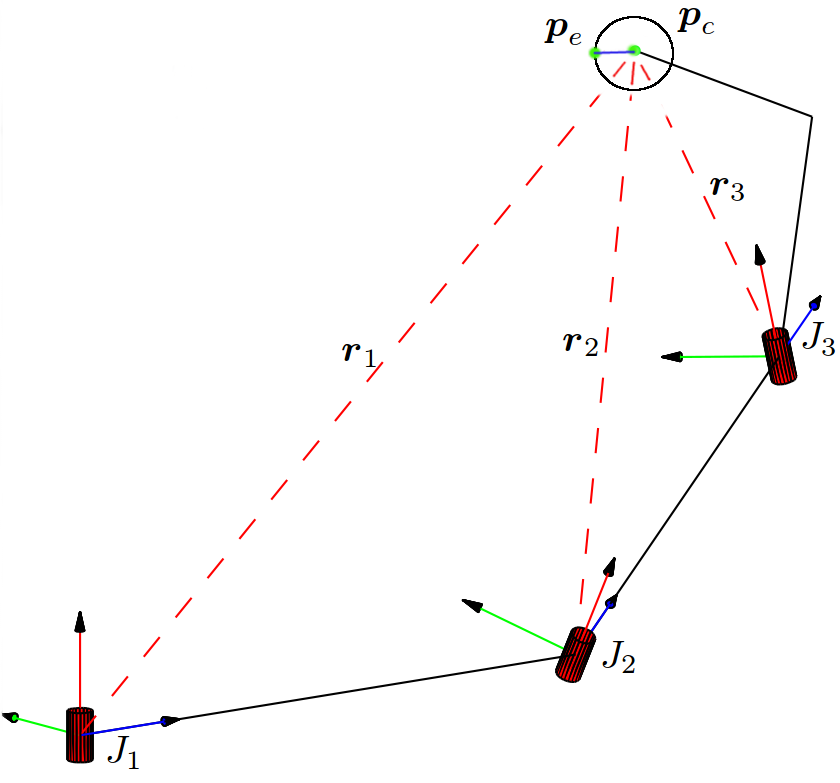
\includegraphics[width=0.8\textwidth]{jacobian1}
  \caption{Three DOF manipulator with a wheel at the end}
\end{figure}

\noindent In this case we get the jacobian matrix corresponding to the center of the wheel (point $p_{c}$) computed with respect to the base frame. However, we're interested  in the jacobian matrix corresponding to the contact point (point $p_{e}$). To obtain the latter we refer to the formula:

\begin{equation}
\boldsymbol{v}_{e} = \boldsymbol{v}_{c} + \boldsymbol{\omega_{c}} \times \boldsymbol{r}_{e, c} 
\end{equation}

\noindent Where $\boldsymbol{r}_{e, c}$ is the wheel radius (blue line in the figure 3).\\

\noindent This can also be written as:

\begin{equation}
\boldsymbol{v}_{e} = \boldsymbol{J}_{c}(\boldsymbol{q})\boldsymbol{\dot{q}} - skew(\boldsymbol{r}_{e, c})\boldsymbol{\omega_{c}}
\end{equation}

\noindent In the formula (16) $\boldsymbol{\omega_{c}}$ accounts for the angular velocity of the frame attached to the center of the wheel (frame of the wheel). $\boldsymbol{\omega_{c}}$ is the sum of all angular velocities
of frames constituting the respective subchain leading to the wheel expressed in the base (0$^{th}$) frame. We can use the following formula to calculate $\boldsymbol{\omega_{c}}$:

\begin{equation}
\boldsymbol{\omega_{c}} = \sum_{j \in subchain}\boldsymbol{{}^0\omega_j^{j-1}} = \sum_{j \in subchain}\boldsymbol{R_{j-1}^{0}}\dot{\boldsymbol{q_{j}}}\boldsymbol{k_{j}^{j-1}} = \sum_{j \in subchain}\dot{\boldsymbol{q_{j}}}\boldsymbol{k_{j}^{0}} + \boldsymbol{\omega_{base}}
\end{equation}

\noindent Where $\boldsymbol{{}^0\omega_j^{j-1}}$ stands for the angular velocity of frame $j$ with respect to frame $j-1$ expressed in frame $0$ and $\boldsymbol{\omega_{base}}$ is given by (13).\\

\noindent Formula (18) is derived based on the following result from kinematics:

\begin{equation}
\boldsymbol{{}^0\omega_n^{0}} = \sum_{j = 1}^{n}\boldsymbol{{}^0\omega_j^{j-1}}
\end{equation}

\noindent We can also write $\boldsymbol{\omega_{c}}$ as:

\begin{equation}
\boldsymbol{\omega_{c}} = \underbrace{\begin{bmatrix}\underbrace{\begin{pmatrix} \boldsymbol{0} & \begin{bmatrix} cos(\beta)cos(\gamma) & -sin(\gamma) & 0 \\ 
                        cos(\beta)sin(\gamma) & cos(\gamma) & 0 \\
                        -sin(\beta) & 0 & 1 \\  \end{bmatrix}    \end{pmatrix}}_{3 \times 6} & \underbrace{\begin{cases}
        \begin{pmatrix} \boldsymbol{k}_{j}^{0} \end{pmatrix} if \ joint \ i \ supports \  wheel \ n \\
        \begin{pmatrix} \boldsymbol{0} \end{pmatrix} \ \ \ \ \ \ \ \ \ \ \ \ \ \ \ \ if \  otherwise
\end{cases}}_{3 \times 15}
\end{bmatrix}}_{\boldsymbol{F}}\begin{bmatrix} q_{0} \\ \vdots \\ q_{20} \end{bmatrix}
\end{equation}

\noindent Inserting $\boldsymbol{F}$ from (20) into (17) gives:

\begin{equation}
\boldsymbol{v}_{e} = \boldsymbol{J}_{c}(\boldsymbol{q})\boldsymbol{\dot{q}} - skew(\boldsymbol{r}_{e, c})\boldsymbol{F}\boldsymbol{\dot{q}}
\end{equation}

\noindent Which finally gives the following expression:

\begin{equation}
\boldsymbol{v}_{e} = \underbrace{(\boldsymbol{J}_{c}(\boldsymbol{q}) - skew(\boldsymbol{r}_{e, c})\boldsymbol{F})}_{Contact Jacobian}\boldsymbol{\dot{q}}
\end{equation}

\noindent Where $\boldsymbol{r}_{e, c}$ stands for the vector from the center of the wheel to the contact point. It can be computed based either on the coordinates of the contact point or the contact normal, hence either
needs to be provided as an argument to the routine computing the jacobian.\\

\noindent The latter way of computing the contact jacobian makes use of the $\boldsymbol{J}_{c}$ matrix which is the jacobian matrix corresponding to the center of the wheel. It can be obtained using a tool like HuMAnS.

\begin{thebibliography}{1}

\bibitem{notes}
 Dimitar Dimitrov, 
 \emph{Slides from Seminar on Multibody Simulation}.
 \url{http://www.aass.oru.se/Research/Learning/drdv_dir/mbs2011/MB_velocity.pdf},
 2012.

\bibitem{notes1}
 Vincent's handnotes. 

\end{thebibliography}

\end{document}
 
